\documentclass[aspectratio=169]{beamer}
\usepackage{ulem}
\usepackage{tikz}
\usepackage{booktabs}
 \usepackage{graphicx,threeparttable,caption}
\usetikzlibrary{shapes,snakes}
\usepackage[beamer,customcolors]{hf-tikz}
\usepackage{nicematrix}
\usepackage{xcolor}
\usepackage{makecell}
\usepackage{array}
\usepackage{csquotes}
\usepackage{csquotes}
\usepackage{minted}
\captionsetup{labelformat=empty,labelsep=none}

\graphicspath{ {./png/} }

\usetikzlibrary{
    arrows,
    arrows.meta,
    shapes,
    positioning,
    shadows,
    trees,
    calc
}

\tikzset{%
    >={Latex[width=2mm,length=2mm]},
    % Specifications for style of nodes:
    plain/.style = {},
    base/.style = {
        plain,
        rectangle, rounded corners, draw=black,
        minimum width=1cm, minimum height=1cm,
        text centered, font=\sffamily\tiny\bfseries,
        fill=white, align=center
    },
    app/.style = {base, ellipse},
    data/.style = {base, fill=gray!30},
    action/.style = {base, circle, fill=red!30},
    note/.style = {app, fill=yellow},
    hl/.style={
    set fill color=red!80!black!40,
    set border color=red!80!black
    }
}


\AtBeginSection[]{
  \begin{frame}
  \vfill
  \centering
  \begin{beamercolorbox}[sep=8pt,center,shadow=true,rounded=true]{title}
    \usebeamerfont{title}\insertsectionhead\par%
  \end{beamercolorbox}
  \vfill
  \end{frame}
}
%\usecolortheme[orchid]{structure}
\usetheme[hideothersubsections]{PaloAlto}
\makeatletter
\patchcmd{\csq@bquote@i}{{#6}}{{\emph{#6}}}{}{}
\makeatother
%\usecolortheme{orchid}
%\usefonttheme{professionalfonts}
\newcommand{\soutthick}[1]{%
   \textcolor{red}{
   \renewcommand{\ULthickness}{1pt}%
      \sout{#1}%
   \renewcommand{\ULthickness}{.4pt}% Resetting to ulem default
   }
}
\newcommand{\centered}[1]{\begin{tabular}{l} #1 \end{tabular}}
\setbeamertemplate{section in toc}[square]
\setbeamertemplate{subsection in toc}[square]
\setbeamertemplate{secion in sidebar}[shaded]
\setbeamertemplate{items}[square]
\setbeamercovered{transparent} 

\title[]{Introduction to Computational Social Science}
\subtitle{Text as data -- does computer understand textual data?}
\author[]{Mikołaj Biesaga\\ \small{\color{blue}{\href{mailto:m.biesaga@uw.edu.pl}{m.biesaga@uw.edu.pl}}}}
\institute{
\includegraphics[width = 4 cm]{uw.png}}
\date{\today}
\begin{document}
\begin{frame}
   \titlepage
\end{frame}

\section[Data]{Data, again}

\begin{frame}
    \frametitle{Structured and Unstructured Data}
    \only<+>{
        \begin{figure}
            
\includegraphics[width = \textwidth]{structured.jpg}
        \end{figure}
    }
    \only<+>{
        \centering
        \begin{columns}[t]
        \begin{column}{.5\textwidth}
            Structured Data:
            \begin{itemize}
                \item can be displayed in rows and columns
                \item numbers, text, dates
                \item requires less storage
                \item easy to manage and analysis
            \end{itemize}
        \end{column}
        \begin{column}{.5\textwidth}
            Unstructured Data:
            \begin{itemize}
                \item can't be displayed in rows and columns
                \item images, audio, video, e-mails, spreadsheets, etc. (fun staff)
                \item requires more storage
                \item extremely hard to manage and analysis
            \end{itemize}
        \end{column}
        \end{columns}
    }
\end{frame}

\begin{frame}
    \frametitle{Data Formats}
    \only<+>{
        Marianna is a 17 years old young lady. Although her main field of interest is physics (especially quantum physics and string theory), she also fancies sports. Her favorite physical activities are fishing and football.
        Marian, on the other hand, is a naughty 15 years old boy who only loves literature, especially Szymborska poems touch his heart.
    }
    \only<+>{
        \textcolor{red}{Marianna} is a \textcolor{blue}{17} years old young lady. Although her main field of interest is \underline{physics} (especially \textbf{quantum physics} and \textbf{string theory}), she also fancies \underline{sport}. Her favorite physical activities are \textbf{fishing} and \textbf{football}.
        \textcolor{red}{Marian}, on the other hand, is a naughty \textcolor{blue}{15} years old boy who only loves \underline{literature}, especially Szymborska \textbf{poems} touches his heart.
    }
    \only<+>{
        \resizebox{\textwidth}{!}{
            \begin{tabular}{l | c | c | c | c | c | c | c | c }
            Name & Sex & Age & Interest A & Interest A1 & Interest A2 & Interest B & Interest B1 & Interest B2\\
            \hline \hline
            Marianna & F & 17 & physics & quantum physics & string theory & sport & fishing & football\\
            Marian & M & 15 & literature & poems & n/a & n/a & n/a & n/a \\
            \end{tabular}}

    }
\end{frame}

\begin{frame}[fragile]{JSON - JavaScript Object Notation}
\begin{minted}[fontsize=\footnotesize]{js}
{   "name": "Marianna",
    "age": 17,
    "interests": [
        {
            "name": "physics",
            "field": [
                "quantum physics",
                "string theory"
            ]
        },
        {
            "name": "sport",
            "field": [
                "fishing",
                "football"
            ]
        }
]}
\end{minted}
\end{frame}

\begin{frame}[fragile]{JSON - JavaScript Object Notation}
\begin{minted}[fontsize=\footnotesize]{js}
{
    "name": "Marian",
    "age": 15,
    "interests": [
        {
            "name": "literature",
            "genre": [
                "poems"
            ]
        }
    ]
}
\end{minted}
\end{frame}

\begin{frame}
    \frametitle{JSON - JavaScript Object Notation}
    \begin{definition}
        \emph{JavaScript Object Notation} is a lightweight text data format that is relatively easy to read for both the human naked eye and computers. Although it derives from JavaScript it is a language-independent data format. JSON is built on two structures: a collection of key-item pairs and an ordered list of values. JSON filenames use .json extension.
    \end{definition}
\begin{definition}
    \emph{JSON Lines} (newline-delimited JSON) is a lightweight text data format that can be processed one record at a time. Each line consists of a JSON. JSON Lines filenames use .jl or .jsonl extensions.
\end{definition}
\end{frame}

\section[Dating]{Ok, Cupid}

\begin{frame}
    \frametitle{What message to write on a dating app?}
    \begin{figure}
        \begin{minipage}{.3\textwidth}
            \vspace{.65cm}
            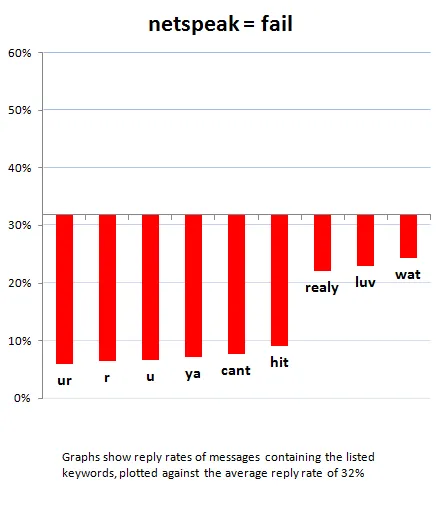
\includegraphics[width = \textwidth]{cupid_1.png}
        \end{minipage}
        \begin{minipage}{.3\textwidth}
            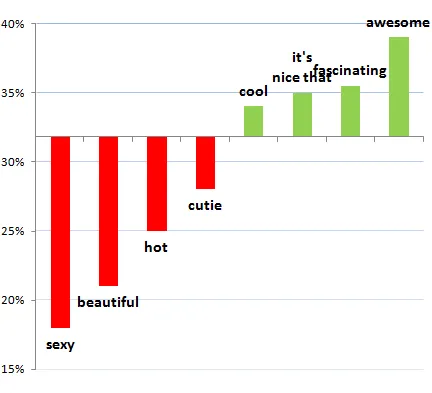
\includegraphics[width = \textwidth]{cupid_2.png}
        \end{minipage}
        \begin{minipage}{.3\textwidth}
            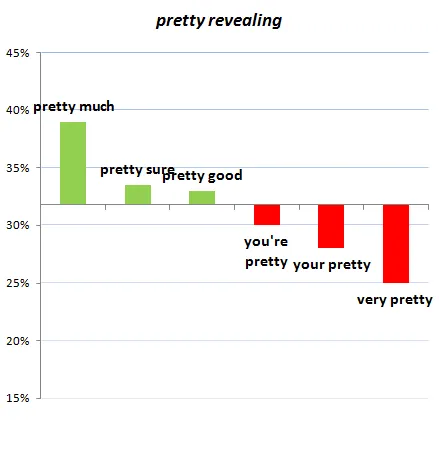
\includegraphics[width = \textwidth]{cupid_3.png}
        \end{minipage}
        \caption*{from \href{https://medium.com/p/2bf680806c72}{\textcolor{blue}{Medium.com}}}
    \end{figure}

\end{frame}

\section[NLP]{Natural Language Processing}

\begin{frame}
    \frametitle{Natural Language Processing}
    \only<+>{
        \begin{definition}
            In a general sense \emph{Natural Language Processing} (NLP) is an analytical approach that uses a set of (usually) computer-based methods to extract meaning, topics, or sentiment from natural language data (written or spoken). In other words, it is a set of computer algorithms that tries to synthesize human language.  \end{definition}
    }
\end{frame}
\begin{frame}
    \frametitle{Sentiment Analysis}
    \only<+>{
        \begin{figure}
            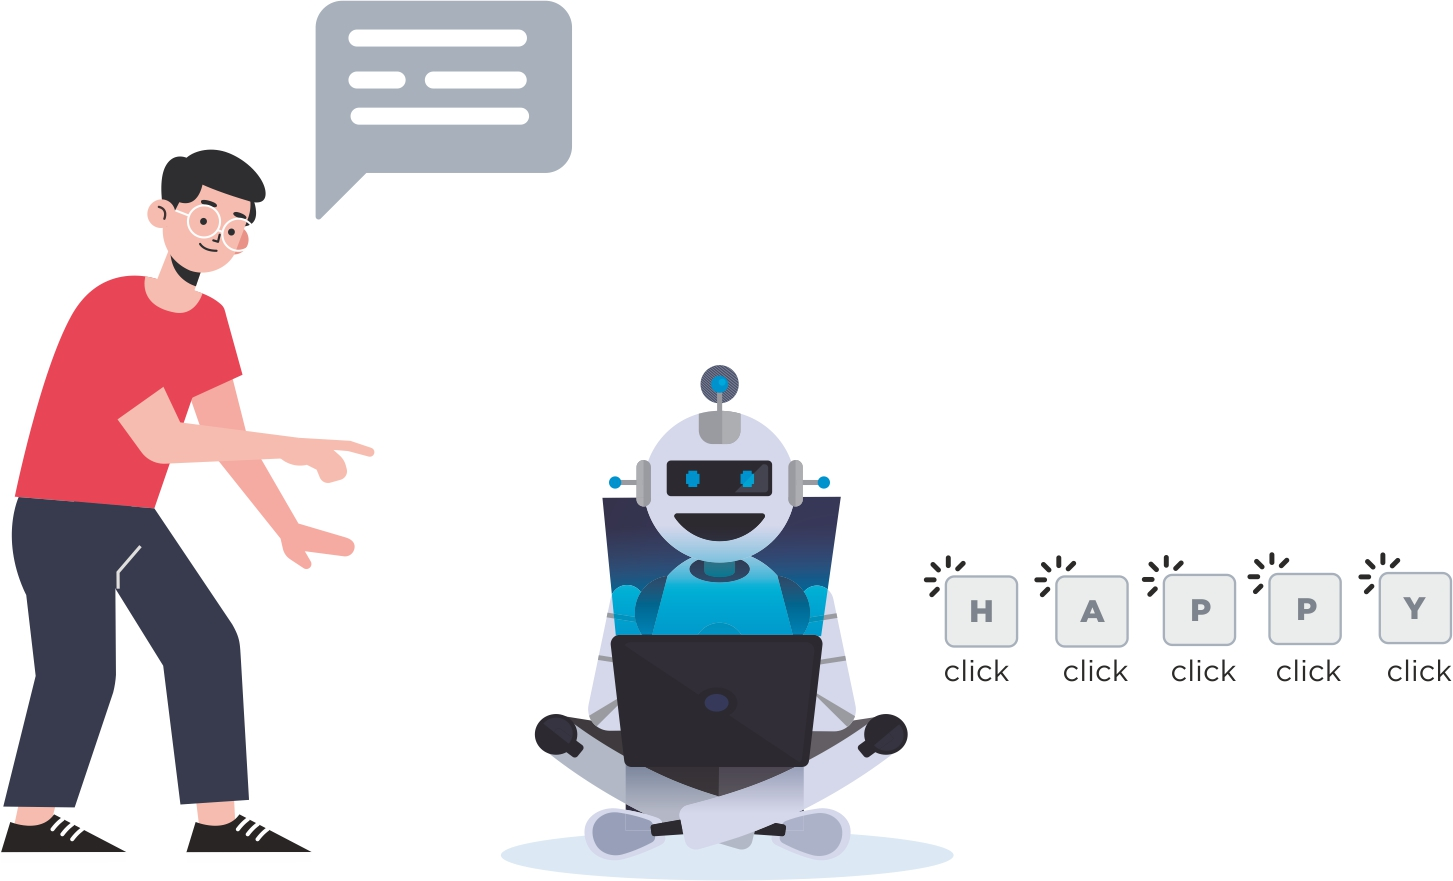
\includegraphics[scale = .7]{png/nlp.jpg}
        \end{figure}
    }
    \only<+>{
        \framesubtitle{Dictionary-based approach}
        \begin{figure}
            \begin{tikzpicture}[>=stealth, text-node/.style={
                rectangle, draw=black, fill=gray!20, text centered, rounded corners}]
                \node[text-node, text width = 3cm] at (0,0) {This movie was so good -- I couldn't stop thinking about it afterward.};
                \node[text-node, text width = 3cm] at (3,4) {The actors were great, but the story was boring and predictable.};
                \node[text-node, text width = 3cm] at (4,2) {It looked amazing, but the characters didn't feel real.};
                \node[text-node, text width = 3cm] at (9,4) {I loved the action scenes; they kept me hooked the whole time.};
                \node[text-node, text width = 3cm] at (8,0) {It felt like the movie was trying too hard to be deep, but it just ended up confusing.};
            \end{tikzpicture}
        \end{figure}
    }
    \only<+>{
        \framesubtitle{Preprocessing}
        \begin{figure}
            \begin{tikzpicture}[>=stealth, text-node/.style={
                rectangle, draw=black, fill=gray!20, text centered, rounded corners, font=\small}]
                \node[text-node, text width = 3cm] (text) at (0,0) {This move was so good -- I couldn't stop thinking about it afterward.};
                \node [text-node, text width = 1.5cm] (token) at (4,0) {This\\ movie\\ was\\ so\\ good\\ --\\ I\\ couldn't\\ stop\\ thinking\\ about\\ it\\ afterward.};
                \node [text-node, text width = 1.5cm] (lemma) at (7,0) {this\\ movie\\ be\\ so\\ good\\ --\\ i\\ cannot\\ stop\\ think\\ about\\ it\\ afterward};
                \node [text-node, text width = 1.5cm] (stop) at (10,0) {\phantom{this}\\ movie\\ be\\ so\\ good\\ \phantom{--}\\ \phantom{I}\\ cannot\\ stop\\ think\\ \phantom{about}\\ \phantom{it}\\ afterward};
                \node at (0,-3.5) {Text};
                \node at (4,-3.5) {Tokenization};
                \node at (7,-3.5) {Lemmatization};
                \node at (10,-3.5) {Stop words};
                \draw [->] (1.7, 0) -- (3,0);
                \draw [->] (5,0) -- (6,0);
                \draw [->] (8,0) -- (9,0);
            \end{tikzpicture}
        \end{figure}
    }
    \only<+>{
        \begin{figure}
            \begin{tikzpicture}[>=stealth, text-node/.style={
                rectangle, draw=black, fill=gray!20, text centered, rounded corners, font=\small}]
                \node [text-node, text width = 1.5cm] (stop) at (0,0) {\phantom{this}\\ movie\\ be\\ so\\ good\\ \phantom{--}\\ \phantom{I}\\ cannot\\ stop\\ think\\ \phantom{about}\\ \phantom{it}\\ afterward};
                \node [text-node, text width = 1.5cm] (stop) at (4,0) {\phantom{this}\\ movie\\ be\\ so\\ \colorbox{green!20}{good}\\ \phantom{--}\\ \phantom{I}\\ cannot\\ stop\\ think\\ \phantom{about}\\ \phantom{it}\\ afterward};
                \node [text-node, text width = 1.5cm, fill = green!20] (stop) at (8,0) {\phantom{this}\\ movie\\ be\\ so\\ good\\ \phantom{--}\\ \phantom{I}\\ cannot\\ stop\\ think\\ \phantom{about}\\ \phantom{it}\\ afterward};
                \node at (8,-3.5) {$sentiment = +.125$};
                \draw [->] (1, 0) -- (3,0);
                \draw [->] (5, 0) -- (7,0);
            \end{tikzpicture}
        \end{figure}
    }
    \only<+>{
        \framesubtitle{Dictionary-based approach}
        \begin{figure}
            \begin{tikzpicture}[>=stealth, text-node/.style={
                rectangle, draw=black, fill=gray!20, text centered, rounded corners}]
                \node[text-node, text width = 3cm, fill = green!20] at (0,0) {This movie was so good -- I couldn't stop thinking about it afterward.};
                \node[text-node, text width = 3cm, fill = red!20] at (3,4) {The actors were great, but the story was boring and predictable.};
                \node[text-node, text width = 3cm, fill = green!20] at (4,2) {It looked amazing, but the characters didn't feel real.};
                \node[text-node, text width = 3cm, fill = green!20] at (9,4) {I loved the action scenes; they kept me hooked the whole time.};
                \node[text-node, text width = 3cm, fill = red!20] at (8,0) {It felt like the movie was trying too hard to be deep, but it just ended up confusing.};
            \end{tikzpicture}
        \end{figure}
    }
    \only<+>{
        \framesubtitle{Machine Learning approach}
        \begin{figure}
            \begin{tikzpicture}[>=stealth, text-node/.style={
                rectangle, draw=black, fill=gray!20, text centered, rounded corners, font=\small}]
                \node[text-node, text width = 3cm] at (0,0) {This move was so good -- I couldn't stop thinking about it afterward.};
                \draw[fill = black] (4,-1) rectangle (6,1);
                \node[text-node, text width = 3cm, fill = green!20] at (10,0) {This move was so good -- I couldn't stop thinking about it afterward.};
                \draw [->] (1.7,0) -- (3.9,0);
                \draw [->] (6.1,0) -- (8.3,0);
                \node at (0,-2.5) {Text};
                \node at (5,-2.5) {Black box};
                \node at (10,-2.5) {$sentiment = +.93$};
            \end{tikzpicture}
        \end{figure}

    }
\end{frame}
\begin{frame}
    \frametitle{Topic Modeling}
    \only<+>{
        \begin{figure}
        \begin{tikzpicture}[>=stealth, scale = .5, small/.style={
            % The shape:
            rectangle,
            % The size:
            minimum size=.75cm,
            % The border
            thick, draw=black,
            % The filling
            fill=white}]
        \foreach \x/\y in {0/0,2/0,8/0}{
          \draw [fill = yellow!30] (\x + 0,0 - \y) rectangle (\x + 1.5,2 - \y);
          \draw (\x + .2,1.4 - \y) rectangle (\x + 1.3,1.9 - \y);
          \foreach \z in {.2,.3,...,1.3}{
            \draw (\x + .2,\z - \y) -- (\x + 1.3,\z - \y);
          }
        }
        \foreach \x/\y in {12/0,6/0,10/0}{
          \draw [fill = red!30] (\x + 0,0 - \y) rectangle (\x + 1.5,2 - \y);
          \draw (\x + .2,1.4 - \y) rectangle (\x + 1.3,1.9 - \y);
          \foreach \z in {.2,.3,...,1.3}{
            \draw (\x + .2,\z - \y) -- (\x + 1.3,\z - \y);
          }
        }
        \foreach \x/\y in {4/0}{
          \draw [fill = green!30] (\x + 0,0 - \y) rectangle (\x + 1.5,2 - \y);
          \draw (\x + .2,1.4 - \y) rectangle (\x + 1.3,1.9 - \y);
          \foreach \z in {.2,.3,...,1.3}{
            \draw (\x + .2,\z - \y) -- (\x + 1.3,\z - \y);
          }
        }
        \foreach \x/\y in {3/4, 3/4.3, 3/4.6}{
          \draw [fill = yellow!30] (\x + 0,0 - \y) rectangle (\x + 1.5,2 - \y);
          \draw (\x + .2,1.4 - \y) rectangle (\x + 1.3,1.9 - \y);
          \foreach \z in {.2,.3,...,1.3}{
            \draw (\x + .2,\z - \y) -- (\x + 1.3,\z - \y);
          }
        }
        \foreach \x/\y in {9/4, 9/4.3, 9/4.6}{
          \draw [fill = red!30] (\x + 0,0 - \y) rectangle (\x + 1.5,2 - \y);
          \draw (\x + .2,1.4 - \y) rectangle (\x + 1.3,1.9 - \y);
          \foreach \z in {.2,.3,...,1.3}{
            \draw (\x + .2,\z - \y) -- (\x + 1.3,\z - \y);
          }
        }
        \foreach \x/\y in {6/4}{
          \draw [fill = green!30] (\x + 0,0 - \y) rectangle (\x + 1.5,2 - \y);
          \draw (\x + .2,1.4 - \y) rectangle (\x + 1.3,1.9 - \y);
          \foreach \z in {.2,.3,...,1.3}{
            \draw (\x + .2,\z - \y) -- (\x + 1.3,\z - \y);
          }
        }
        \draw (.75,0) [->] -- (3.65, -2);
        \draw (2.75,0) [->] -- (3.75, -2);
        \draw (8.75,0) [->] -- (3.85, -2);
        \draw (4.75,0) [->] -- (6.75, -2);
        \draw (6.75,0) [->] -- (9.65, -2);
        \draw (10.75,0) [->] -- (9.75, -2);
        \draw (12.75,0) [->] -- (9.85, -2);
    
        \draw [fill = yellow!30] (3, -8.6) rectangle (4.5, -6.6);
        \draw [fill = red!30] (9, -8.6) rectangle (10.5, -6.6);
    
        \draw (3.75, -4.8) -- ++(270:1.6) -- ++(0:6) -- ++(90:1.6);
    
        \node at (16,1) {Corpus};
        \node at (16,-3) {Separated Topics};
        \node at (16,-7.3) {Identified Narratives};
    
        \end{tikzpicture}
    \end{figure}
    }
    \only<+>{
        \begin{figure}
            \begin{tikzpicture}[>=stealth, text-node/.style={
                rectangle, draw=black, fill=gray!20, text centered, rounded corners}]
                \node[text-node, text width = 3cm] at (0,0) {Fear of failure leads to failure.};
                \node[text-node, text width = 3cm] at (3,4) {If we do not face our fears, our fears will chase us forever.};
                \node[text-node, text width = 3cm] at (4,1.5) {Be brave. Take risks. Nothing can substitute experience.};
                \node[text-node, text width = 3cm] at (9,4) {We do not need to explain our love. We only need to show it.};
                \node[text-node, text width = 3cm] at (8,0) {Love yourself first because this is the person you are going to spend the rest of your life with.};
            \end{tikzpicture}
        \end{figure}
    }
\end{frame}


\begin{frame}
    \frametitle{For the class in two weeks}
    \begin{itemize}
        \item  Milgram, S. (1967). The small-world problem. Psychology Today, 1(1), 61–67.
        \item  Lazer, D., Pentland, A. (Sandy), Adamic, L., Aral, S., Barabasi, A. L., Brewer, D., Christakis, N., Contractor, N., Fowler, J., Gutmann, M., Jebara, T., King, G., Macy, M., Roy, D., \& Van Alstyne, M. (2009). Life in the network: The coming age of computational social science. Science, 323(5915), 721–723. \href{https://doi.org/10.1126/science.1167742}{\textcolor{blue}{https://doi.org/10.1126/science.1167742}}.

    \end{itemize}
\end{frame}
\end{document}
